% This is part of Un soupçon de mathématique sans être agressif pour autant
% Copyright (c) 2015
%   Laurent Claessens
% See the file fdl-1.3.txt for copying conditions.

\begin{exercice}\label{exo2smath-0301}

 Parmi les patrons suivants, lesquels sont des patrons de prismes droits ? De cylindres ?  Pour ceux qui ne le sont pas, expliquer pourquoi.

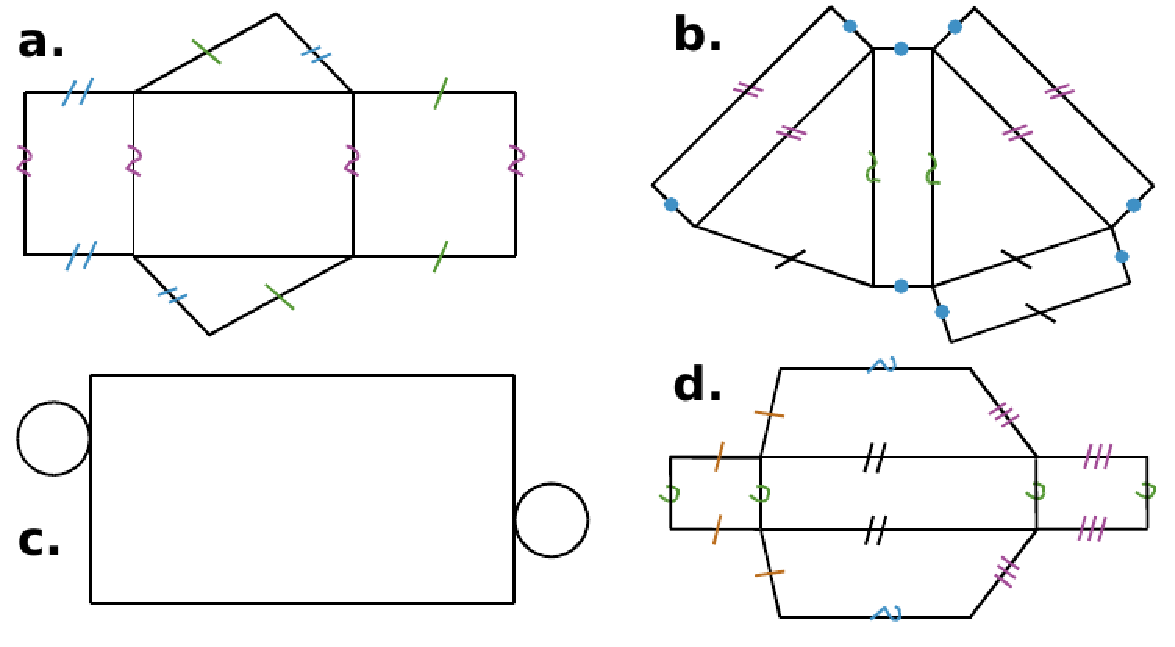
\includegraphics[width=8cm]{despatrons.pdf}

\corrref{2smath-0301}
\end{exercice}
